\begin{figure}[!tbp]
\centering 
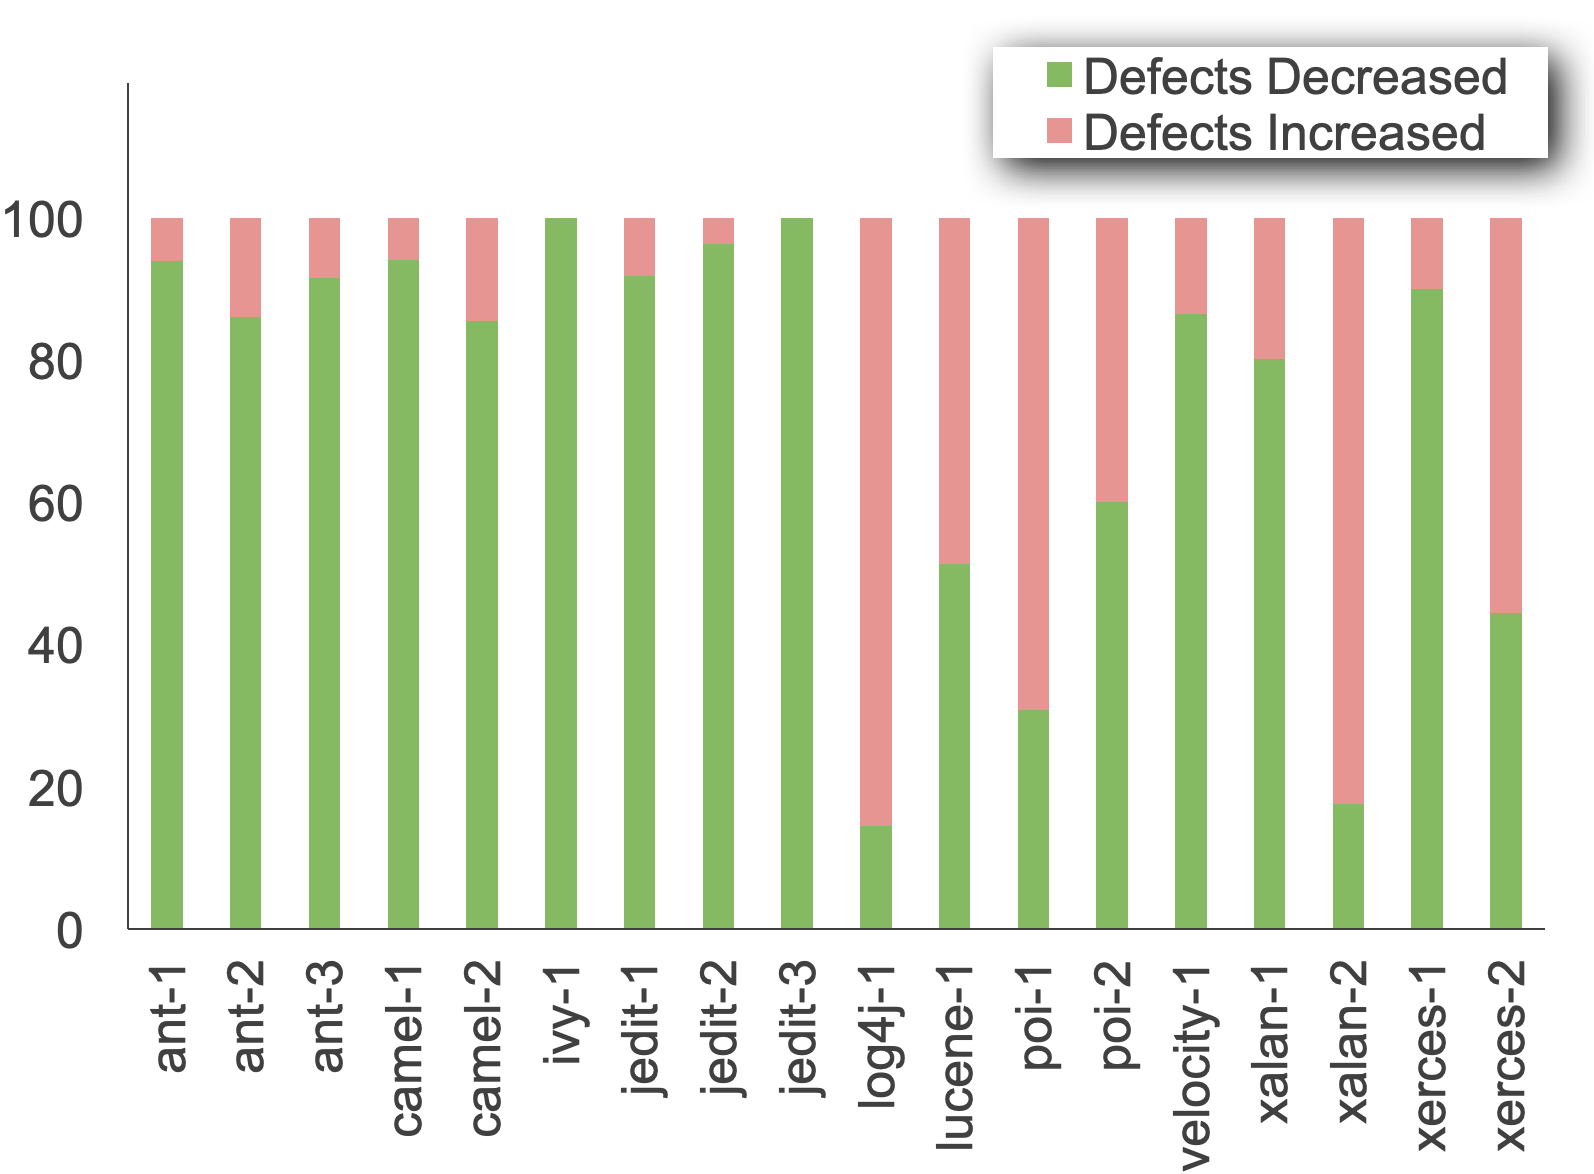
\includegraphics[width=0.75\linewidth]{rq2_3.png}
\caption{A count of total number \textit{defects reduced} and \textit{defects increased} as a result each planners' recommendations. The overlaps are again categorized into four ranges for every dataset (denoted by $min\leq~Overlap<max$). For each of the overlap ranges, we count the total number of \textit{defects reduced} and \textit{defects increased} in the validation set for the classes that were defective in the test set as a result of overlap between the planner's recommendation and the developers changes that fell in the given range}
\label{fig:rq2_1}
\end{figure}